%% Esqueleto base de la presentacion
%%% No agregar las paginas con un include
%%% Lo que quieran aportar deben ser usuarios del TRAC

\documentclass{beamer}
\usepackage[english,activeacute]{babel}
\usepackage[utf8]{inputenc}
\usepackage{listings}
\usepackage{algorithmic}
\usepackage{color}

\definecolor{gray2}{rgb}{100,100,100}
\definecolor{red}{rgb}{255,0,0}
\definecolor{blue}{rgb}{0,0,255}
\definecolor{gray97}{gray}{.97}
\definecolor{gray75}{gray}{.75}
\definecolor{gray45}{gray}{.45}

\newcommand{\blue}{\textcolor{blue}}
\newcommand{\red}{\textcolor{red}}
\newcommand{\green}{\textcolor{green}}


\usetheme[pageofpages=of,% String used between the current page and the
                         % total page count.
          alternativetitlepage=true,% Use the fancy title page.
          titlepagelogo=img/logo,% Logo for the first page.
          watermark=,% Watermark used in every page.
          watermarkheight=100px,% Height of the watermark.
          watermarkheightmult=4,% The watermark image is 4 times bigger
                                % than watermarkheight.
          ]{Torino}

\usecolortheme{nouvelle}


\lstset{ frame=Ltb,
     framerule=0pt,
     aboveskip=0.5cm,
     framextopmargin=3pt,
     framexbottommargin=3pt,
     framexleftmargin=0.4cm,
     framesep=0pt,
     rulesep=.4pt,
     backgroundcolor=\color{gray97},
     rulesepcolor=\color{black},
     %
     stringstyle=\ttfamily,
     showstringspaces = false,
     basicstyle=\tiny\ttfamily,
     %commentstyle=\color{gray45},
     %keywordstyle=\bfseries,
     %
     numbers=left,
     numbersep=13pt,
     numberstyle=\tiny,
     numberfirstline = false,
     breaklines=true,
	 emph = {[1]\_\_device\_\_,\_\_global\_\_,\_\_syncthreads,pthread\_create,pthread\_join,pragma,omp,parallel,private, threadIdx, blockDim, blockIdx,cudaThreadSynchronize},
	 emphstyle={[1]\color{blue}},
   }

% minimizar fragmentado de listados
\lstnewenvironment{listing}[1][]
   {\lstset{#1}\pagebreak[0]}{\pagebreak[0]}

\lstdefinestyle{consola}
   {basicstyle=\scriptsize\bf\ttfamily,
    backgroundcolor=\color{gray75},
   }
\lstdefinestyle{C}
   {language=C,
   }

\author[C. Maureira]{\large Cristián Maureira Fredes\\\normalsize \textcolor{gray}{cmaureir@csrg.cl}}
\title[n-body visualization]{N-body problem visualization.}
\subtitle{Using OpenGL}
\institute[UTFSM]{Departamento de Informática\\Universidad Técnica Federico Santa María}
\date{\today}

\begin{document}
\begin{frame}[t,plain]
\titlepage
\end{frame}
\frame
{
\frametitle{N-body problem}
\begin{block}{Definition}
    Predict the \underline{movement} of a \underline{celestial objects} group,
    which are \underline{interacting} with each other \underline{gravitationally}.
\end{block}
}

\frame
{
\frametitle{N-body problem}
\begin{itemize}
    \item Dynamic simulation of a particle system.
    \item Applications.
    \begin{itemize}
        \item Fluid mechanics
        \item Astrophysics
        \item Stellar dynamics
        \item Video games
        \item etc.
    \end{itemize}
\end{itemize}
}


\frame
{
\frametitle{N-body problem}
Critical sections:
\begin{itemize}
    \item Initial positions.
    \item Integration method.
    \item Force calculation.
\end{itemize}
}


\frame
{
\frametitle{N-body problem}

\begin{itemize}
    \item Force calculation.
    \begin{itemize}
        \item Initial positions $x_i$.
        \item Initial velocities $v_i$.
        \item $1 \leq i \leq N$
    \end{itemize}
    $$f_{ij} =G \cdot \frac{m_i \cdot m_j}{||r_{ij}||^{2}} \cdot \frac{r_{ij}}{||r_ij||}$$
    \begin{itemize}
        \item $m_i$ and $m_j$ masses of the $i$ and $j$ bodies.
        \item $r_{ij} = (x_j - x_i )$ distance vector between the $i$ and $j$ bodies.
        \item $G$, gravitational constant. ($6,67428 \times 10^{-11} m^{3} kg^{-1} s^{-2}$)
    \end{itemize}
\end{itemize}
}

\begin{frame}
    \frametitle{Implementation}
    \begin{itemize}
        \item Program structure:
        \begin{itemize}
            \item Read information files.
            \item GLut initialization.
            \item Display.
            \item Reshape.
        \end{itemize}
    \end{itemize}
\end{frame}

\begin{frame}
    \frametitle{Implementation}
    \begin{itemize}
        \item \texttt{GL\_POINTS}
    \end{itemize}
    \begin{figure}
        \begin{center}
           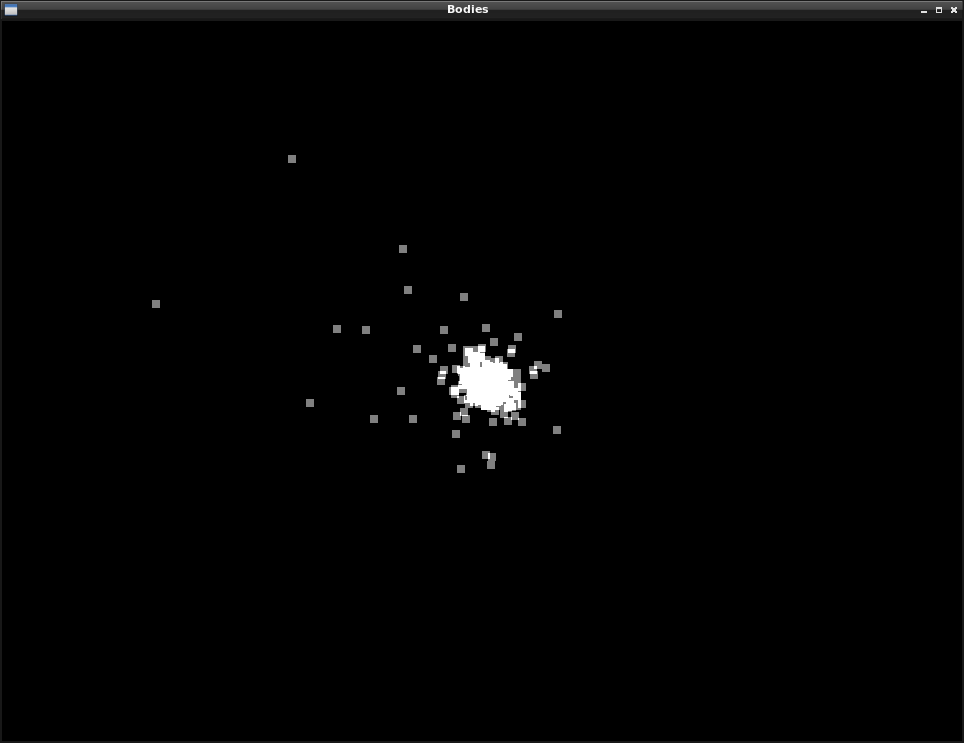
\includegraphics[width=0.6\textwidth]{img/bodies_sin_textura} 
        \end{center}
        \caption{Simple \texttt{GL\_POINTS} visualization (256)}
    \end{figure}
\end{frame}

\begin{frame}
    \frametitle{Implementation}
    \begin{itemize}
        \item \texttt{GL\_POINTS} + \texttt{GL\_TEXTURE\_2D}
    \end{itemize}
    \begin{figure}
        \begin{center}
           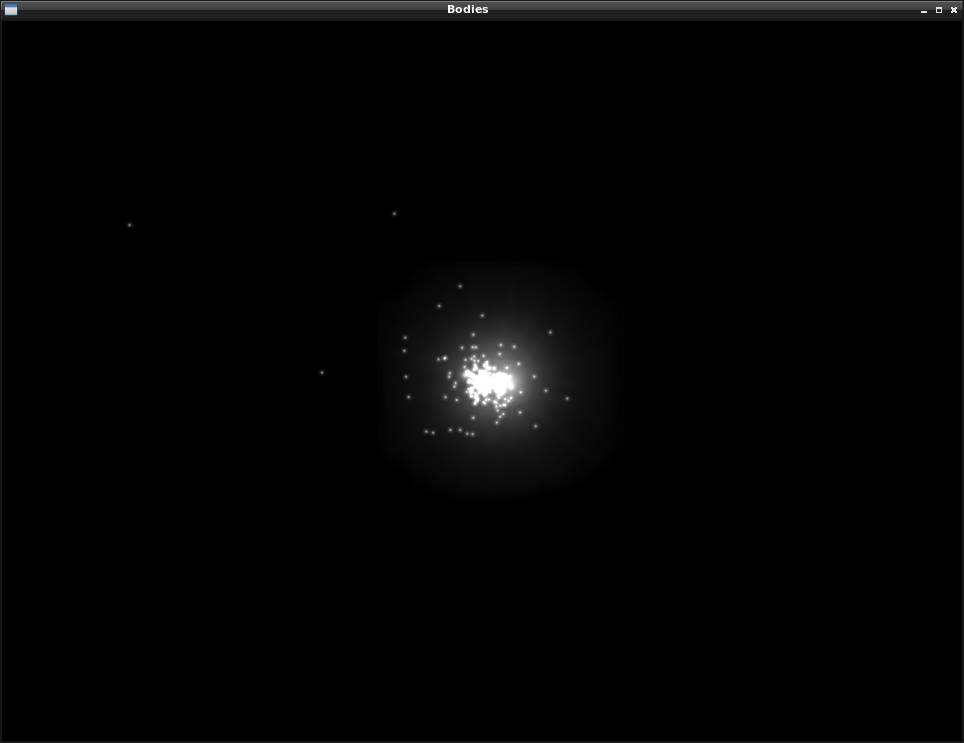
\includegraphics[width=0.6\textwidth]{img/bodies_con_textura} 
        \end{center}
        \caption{Simple \texttt{GL\_POINTS} visualization (256)}
    \end{figure}
\end{frame}

\begin{frame}
    \frametitle{Implementation}
    \begin{figure}
        \begin{center}
           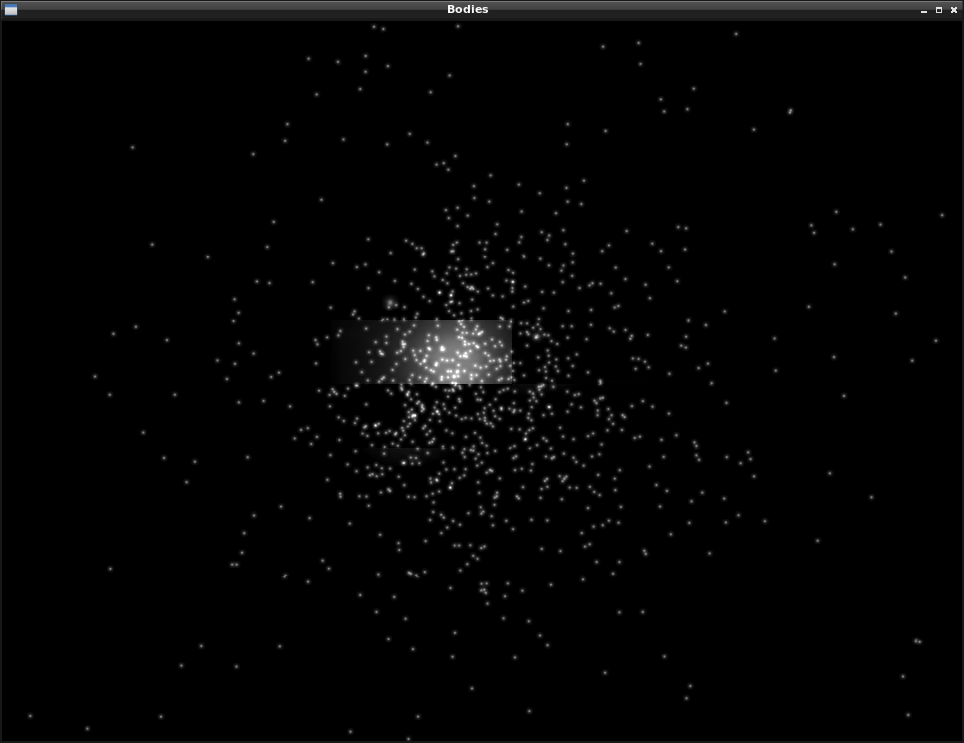
\includegraphics[width=0.7\textwidth]{img/bodies_con_textura_1024-2} 
        \end{center}
        \caption{Final visualization (1024)}
    \end{figure}
\end{frame}

\begin{frame}
    \frametitle{Implementation}
    \framesubtitle{Camera}
    \begin{figure}
        \begin{center}
           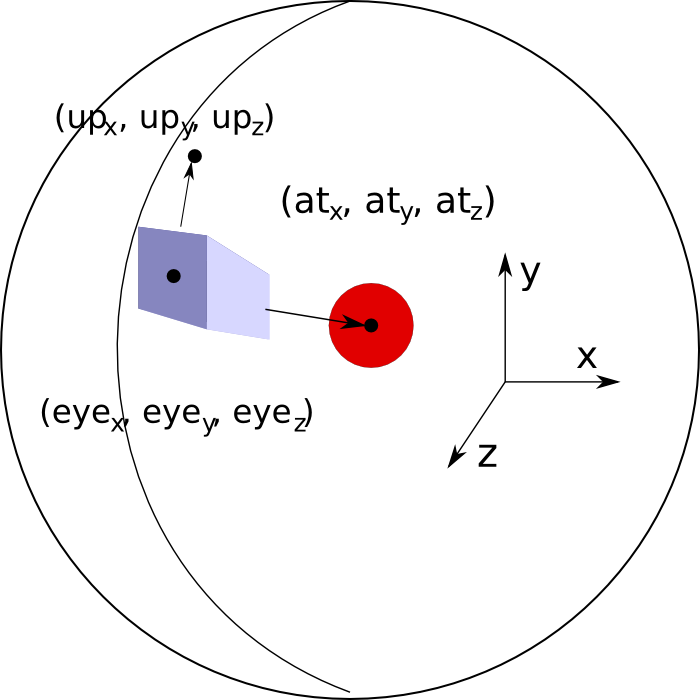
\includegraphics[width=0.5\textwidth]{img/camera} 
        \end{center}
        \caption{GluLookAt}
    \end{figure}
\end{frame}

\begin{frame}
    \frametitle{Implementation}
    \framesubtitle{Spherical coordinates}
    \begin{columns}
        \begin{column}{0.5\textwidth}
            \begin{eqnarray}
                (r, \theta, \varphi) \nonumber \\ \nonumber \\
                r = \sqrt{x^{2} + y^{2} + z^{2}} \nonumber\\
                \theta  = \arccos \left( \frac{z}{r}\right) \nonumber \\
                \varphi = \arccos \left( \frac{y}{x}\right) \nonumber
            \end{eqnarray}
        \end{column}
        \begin{column}{0.5\textwidth}
            \begin{eqnarray}
                (x, y, z) \nonumber \\ \nonumber \\
                x = r \cos{\varphi} \sin{\theta} \nonumber \\
                y = r \sin{\varphi} \sin{\theta} \nonumber \\
                z = r \cos{\theta}  \nonumber
            \end{eqnarray}
        \end{column}
    \end{columns}
\end{frame}

\begin{frame}
    \frametitle{Conclusions}
    \begin{itemize}
        \item Widely used in scientific research.
        \item The utility of the camera move.
        \item Future improvment.
        \item Modularization.
    \end{itemize}
\end{frame}

\begin{frame}[t,plain]
\titlepage
\end{frame}
\end{document}
